\chapter{External specification}
\begin{itemize}
\item hardware and software requirements
\item installation procedure
\item activation procedure
\item types of users
\item user manual
\item system administration
\item security issues
\item example of usage
\item working scenarios (with screenshots or output files)
\end{itemize}

\section{Hardware and software requirements}

Depending on whether one wants to use the user interface via a web browser or host the server themselves there are different requirements for each part.

\subsection{Browser}

The user interface requires a modern browser with JavaScript enabled. It is possible to use the system without JS, but theme switching and dropdowns in the navigation bar will not work.

On desktop the latest stable versions of the following browsers are supported:

\begin{itemize}
    \item Google Chrome
    \item Microsoft Edge
    \item Firefox and Firefox ESR
    \item Opera
    \item Safari (macOS only)
\end{itemize}

On Android and iOS support is restricted to the latest stable versions of:

\begin{itemize}
    \item Google Chrome
    \item Firefox
    \item Safari (iOS only)
    \item Android Browser and WebView (Android only)
\end{itemize}

Different and older browsers may work, but compatibility is not guaranteed.

\subsection{Server software} \label{chap:server-soft}

The server software requires the following external software to be installed:

\begin{itemize}
    \item Node.js 18.x or newer (not as a \href{https://snapcraft.io/node}{snap})
    \item MongoDB 6.0
    \item Docker Engine 20.10
    \item nginx 1.23.2 or newer
\end{itemize}

Supported operating systems:

% https://github.com/ranisalt/node-argon2/tree/v0.30.3#prebuilt-binaries
\begin{itemize}
    \item Ubuntu 20.04 or newer (x86-64, arm64)
    \item macOS 11 (x86-64), 12 or newer (x86-64, arm64)
    \item Windows 10 1809 or newer (x86-64)
    \item Windows Server 2019 or newer (x86-64)
\end{itemize}

It may be possible to run the server on other operating systems and architectures as long as the required software can be installed. These unsupported systems, however, will probably require \href{https://github.com/ranisalt/node-argon2/tree/v0.30.3#before-installing}{additional installation steps} related to \texttt{argon2} package setup.

\textbf{Warning:} Challenge Docker images must be compatible with the server architecture. Images presented in this project support only x86-64.

\section{Server installation}

The process of server software installation and configuration can be summarised in the following steps:

\begin{enumerate}
    \item Install the required software as described in section \ref{chap:server-soft}.
    \item Obtain the code from GitHub:\\
    \mintinline{bash}|git clone https://github.com/krzysdz/inz.git|
    \item Navigate to the downloaded project directory:\\
    \mintinline{bash}|cd inz|
    \item Install required npm packages:\\
    \mintinline{bash}|npm install --omit=dev|
    \item Configure MongoDB as a replica set (\href{https://www.mongodb.com/docs/manual/tutorial/deploy-replica-set/}{tutorial}).
    \item Configure the DNS to point the main domain and the challenges domain to the server. Example DNS configuration:
    \begin{minted}{DNSLexer.py:DNSLexer -x}
main-ui.com.        60  IN A        127.0.0.1
*.challenges.com.   60  IN CNAME    main-ui.com.
    \end{minted}
    \item Obtain TLS certificate for the main domain and the challenges domain. One certificate should cover both domains (the second one with wildcard).\\
    The key and certificate files should be placed in \texttt{nginx/certs} and named according to instructions from the \texttt{README} file in that directory.
    \item Adjust values in the \texttt{config.js} file.
    \item Start nginx with prefix set to \texttt{./nginx} and configuration \texttt{nginx/conf/nginx.conf}:\\
    \mintinline{bash}|nginx -p ./nginx -c ./nginx/conf/nginx.conf|
    \item Set \texttt{NODE\_ENV} to production:

    Bash/dash/zsh/csh:\\
    \mintinline{bash}|export NODE_ENV="production"|

    Powershell:\\
    \mintinline{pwsh}|$env:NODE_ENV="production"|
    \item Start the server:\\
    \mintinline{bash}|node index.js|
\end{enumerate}


\begin{figure}
\centering
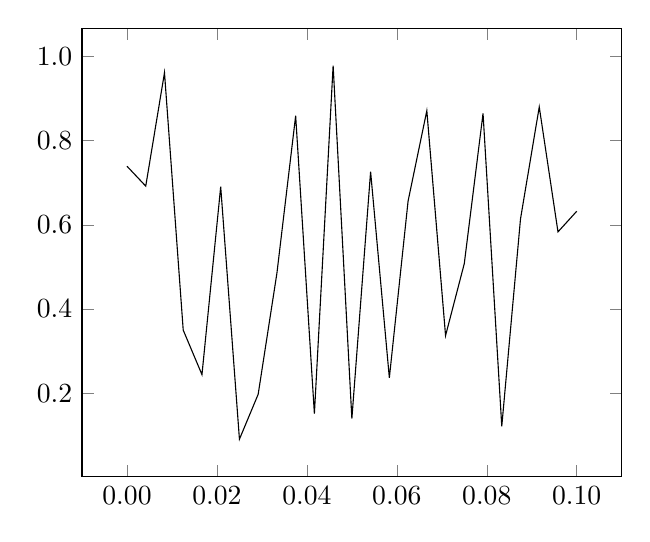
\begin{tikzpicture}
\begin{axis}[
    y tick label style={
        /pgf/number format/.cd,
            fixed,
            fixed zerofill, % 1.0 zamiast 1
            precision=1,
        /tikz/.cd
    },
    x tick label style={
        /pgf/number format/.cd,
            fixed,
            fixed zerofill,
            precision=2,
        /tikz/.cd
    }
]
\addplot [domain=0.0:0.1] {rnd};
\end{axis}
\end{tikzpicture}
\caption{Figure caption (below the figure).}
\label{fig:2}
\end{figure}

%%%%%%%%%%%%%%%%%%%%%
% FIGURE FROM FILE
%
%\begin{figure}
%\centering
%
\includegraphics[width=0.5\textwidth]{./graf/politechnika_sl_logo_bw_pion_en.pdf}
%\caption{Caption of a figure is always below the figure.}
%\label{fig:label}
%\end{figure}
%Fig. \ref{fig:label} presents …
%%%%%%%%%%%%%%%%%%%%%
%
%%%%%%%%%%%%%%%%%%%%
%% SUBFIGURES
%
%\begin{figure}
%\centering
%\begin{subfigure}{0.4\textwidth}
%    
\includegraphics[width=\textwidth]{./graf/politechnika_sl_logo_bw_pion_en.pdf}
%    \caption{Upper left figure.}
%    \label{fig:upper-left}
%\end{subfigure}
%\hfill
%\begin{subfigure}{0.4\textwidth}
%    
\includegraphics[width=\textwidth]{./graf/politechnika_sl_logo_bw_pion_en.pdf}
%    \caption{Upper right figure.}
%    \label{fig:upper-right}
%\end{subfigure}
%
%\begin{subfigure}{0.4\textwidth}
%    
\includegraphics[width=\textwidth]{./graf/politechnika_sl_logo_bw_pion_en.pdf}
%    \caption{Lower left figure.}
%    \label{fig:lower-left}
%\end{subfigure}
%\hfill
%\begin{subfigure}{0.4\textwidth}
%    
\includegraphics[width=\textwidth]{./graf/politechnika_sl_logo_bw_pion_en.pdf}
%    \caption{Lower right figure.}
%    \label{fig:lower-right}
%\end{subfigure}
%
%\caption{Common caption for all subfigures.}
%\label{fig:subfigures}
%\end{figure}
%Fig. \ref{fig:subfigures} presents very important information, eg. Fig. \ref{fig:upper-right} is an upper right subfigure.
%%%%%%%%%%%%%%%%%%%%%
